
% Default to the notebook output style

    


% Inherit from the specified cell style.




    
\documentclass[11pt]{article}

    
    
    \usepackage[T1]{fontenc}
    % Nicer default font (+ math font) than Computer Modern for most use cases
    \usepackage{mathpazo}

    % Basic figure setup, for now with no caption control since it's done
    % automatically by Pandoc (which extracts ![](path) syntax from Markdown).
    \usepackage{graphicx}
    % We will generate all images so they have a width \maxwidth. This means
    % that they will get their normal width if they fit onto the page, but
    % are scaled down if they would overflow the margins.
    \makeatletter
    \def\maxwidth{\ifdim\Gin@nat@width>\linewidth\linewidth
    \else\Gin@nat@width\fi}
    \makeatother
    \let\Oldincludegraphics\includegraphics
    % Set max figure width to be 80% of text width, for now hardcoded.
    \renewcommand{\includegraphics}[1]{\Oldincludegraphics[width=.8\maxwidth]{#1}}
    % Ensure that by default, figures have no caption (until we provide a
    % proper Figure object with a Caption API and a way to capture that
    % in the conversion process - todo).
    \usepackage{caption}
    \DeclareCaptionLabelFormat{nolabel}{}
    \captionsetup{labelformat=nolabel}

    \usepackage{adjustbox} % Used to constrain images to a maximum size 
    \usepackage{xcolor} % Allow colors to be defined
    \usepackage{enumerate} % Needed for markdown enumerations to work
    \usepackage{geometry} % Used to adjust the document margins
    \usepackage{amsmath} % Equations
    \usepackage{amssymb} % Equations
    \usepackage{textcomp} % defines textquotesingle
    % Hack from http://tex.stackexchange.com/a/47451/13684:
    \AtBeginDocument{%
        \def\PYZsq{\textquotesingle}% Upright quotes in Pygmentized code
    }
    \usepackage{upquote} % Upright quotes for verbatim code
    \usepackage{eurosym} % defines \euro
    \usepackage[mathletters]{ucs} % Extended unicode (utf-8) support
    \usepackage[utf8x]{inputenc} % Allow utf-8 characters in the tex document
    \usepackage{fancyvrb} % verbatim replacement that allows latex
    \usepackage{grffile} % extends the file name processing of package graphics 
                         % to support a larger range 
    % The hyperref package gives us a pdf with properly built
    % internal navigation ('pdf bookmarks' for the table of contents,
    % internal cross-reference links, web links for URLs, etc.)
    \usepackage{hyperref}
    \usepackage{longtable} % longtable support required by pandoc >1.10
    \usepackage{booktabs}  % table support for pandoc > 1.12.2
    \usepackage[inline]{enumitem} % IRkernel/repr support (it uses the enumerate* environment)
    \usepackage[normalem]{ulem} % ulem is needed to support strikethroughs (\sout)
                                % normalem makes italics be italics, not underlines
    

    
    
    % Colors for the hyperref package
    \definecolor{urlcolor}{rgb}{0,.145,.698}
    \definecolor{linkcolor}{rgb}{.71,0.21,0.01}
    \definecolor{citecolor}{rgb}{.12,.54,.11}

    % ANSI colors
    \definecolor{ansi-black}{HTML}{3E424D}
    \definecolor{ansi-black-intense}{HTML}{282C36}
    \definecolor{ansi-red}{HTML}{E75C58}
    \definecolor{ansi-red-intense}{HTML}{B22B31}
    \definecolor{ansi-green}{HTML}{00A250}
    \definecolor{ansi-green-intense}{HTML}{007427}
    \definecolor{ansi-yellow}{HTML}{DDB62B}
    \definecolor{ansi-yellow-intense}{HTML}{B27D12}
    \definecolor{ansi-blue}{HTML}{208FFB}
    \definecolor{ansi-blue-intense}{HTML}{0065CA}
    \definecolor{ansi-magenta}{HTML}{D160C4}
    \definecolor{ansi-magenta-intense}{HTML}{A03196}
    \definecolor{ansi-cyan}{HTML}{60C6C8}
    \definecolor{ansi-cyan-intense}{HTML}{258F8F}
    \definecolor{ansi-white}{HTML}{C5C1B4}
    \definecolor{ansi-white-intense}{HTML}{A1A6B2}

    % commands and environments needed by pandoc snippets
    % extracted from the output of `pandoc -s`
    \providecommand{\tightlist}{%
      \setlength{\itemsep}{0pt}\setlength{\parskip}{0pt}}
    \DefineVerbatimEnvironment{Highlighting}{Verbatim}{commandchars=\\\{\}}
    % Add ',fontsize=\small' for more characters per line
    \newenvironment{Shaded}{}{}
    \newcommand{\KeywordTok}[1]{\textcolor[rgb]{0.00,0.44,0.13}{\textbf{{#1}}}}
    \newcommand{\DataTypeTok}[1]{\textcolor[rgb]{0.56,0.13,0.00}{{#1}}}
    \newcommand{\DecValTok}[1]{\textcolor[rgb]{0.25,0.63,0.44}{{#1}}}
    \newcommand{\BaseNTok}[1]{\textcolor[rgb]{0.25,0.63,0.44}{{#1}}}
    \newcommand{\FloatTok}[1]{\textcolor[rgb]{0.25,0.63,0.44}{{#1}}}
    \newcommand{\CharTok}[1]{\textcolor[rgb]{0.25,0.44,0.63}{{#1}}}
    \newcommand{\StringTok}[1]{\textcolor[rgb]{0.25,0.44,0.63}{{#1}}}
    \newcommand{\CommentTok}[1]{\textcolor[rgb]{0.38,0.63,0.69}{\textit{{#1}}}}
    \newcommand{\OtherTok}[1]{\textcolor[rgb]{0.00,0.44,0.13}{{#1}}}
    \newcommand{\AlertTok}[1]{\textcolor[rgb]{1.00,0.00,0.00}{\textbf{{#1}}}}
    \newcommand{\FunctionTok}[1]{\textcolor[rgb]{0.02,0.16,0.49}{{#1}}}
    \newcommand{\RegionMarkerTok}[1]{{#1}}
    \newcommand{\ErrorTok}[1]{\textcolor[rgb]{1.00,0.00,0.00}{\textbf{{#1}}}}
    \newcommand{\NormalTok}[1]{{#1}}
    
    % Additional commands for more recent versions of Pandoc
    \newcommand{\ConstantTok}[1]{\textcolor[rgb]{0.53,0.00,0.00}{{#1}}}
    \newcommand{\SpecialCharTok}[1]{\textcolor[rgb]{0.25,0.44,0.63}{{#1}}}
    \newcommand{\VerbatimStringTok}[1]{\textcolor[rgb]{0.25,0.44,0.63}{{#1}}}
    \newcommand{\SpecialStringTok}[1]{\textcolor[rgb]{0.73,0.40,0.53}{{#1}}}
    \newcommand{\ImportTok}[1]{{#1}}
    \newcommand{\DocumentationTok}[1]{\textcolor[rgb]{0.73,0.13,0.13}{\textit{{#1}}}}
    \newcommand{\AnnotationTok}[1]{\textcolor[rgb]{0.38,0.63,0.69}{\textbf{\textit{{#1}}}}}
    \newcommand{\CommentVarTok}[1]{\textcolor[rgb]{0.38,0.63,0.69}{\textbf{\textit{{#1}}}}}
    \newcommand{\VariableTok}[1]{\textcolor[rgb]{0.10,0.09,0.49}{{#1}}}
    \newcommand{\ControlFlowTok}[1]{\textcolor[rgb]{0.00,0.44,0.13}{\textbf{{#1}}}}
    \newcommand{\OperatorTok}[1]{\textcolor[rgb]{0.40,0.40,0.40}{{#1}}}
    \newcommand{\BuiltInTok}[1]{{#1}}
    \newcommand{\ExtensionTok}[1]{{#1}}
    \newcommand{\PreprocessorTok}[1]{\textcolor[rgb]{0.74,0.48,0.00}{{#1}}}
    \newcommand{\AttributeTok}[1]{\textcolor[rgb]{0.49,0.56,0.16}{{#1}}}
    \newcommand{\InformationTok}[1]{\textcolor[rgb]{0.38,0.63,0.69}{\textbf{\textit{{#1}}}}}
    \newcommand{\WarningTok}[1]{\textcolor[rgb]{0.38,0.63,0.69}{\textbf{\textit{{#1}}}}}
    
    
    % Define a nice break command that doesn't care if a line doesn't already
    % exist.
    \def\br{\hspace*{\fill} \\* }
    % Math Jax compatability definitions
    \def\gt{>}
    \def\lt{<}
    % Document parameters
    \title{Final\_Project\_draft}
    
    
    

    % Pygments definitions
    
\makeatletter
\def\PY@reset{\let\PY@it=\relax \let\PY@bf=\relax%
    \let\PY@ul=\relax \let\PY@tc=\relax%
    \let\PY@bc=\relax \let\PY@ff=\relax}
\def\PY@tok#1{\csname PY@tok@#1\endcsname}
\def\PY@toks#1+{\ifx\relax#1\empty\else%
    \PY@tok{#1}\expandafter\PY@toks\fi}
\def\PY@do#1{\PY@bc{\PY@tc{\PY@ul{%
    \PY@it{\PY@bf{\PY@ff{#1}}}}}}}
\def\PY#1#2{\PY@reset\PY@toks#1+\relax+\PY@do{#2}}

\expandafter\def\csname PY@tok@w\endcsname{\def\PY@tc##1{\textcolor[rgb]{0.73,0.73,0.73}{##1}}}
\expandafter\def\csname PY@tok@c\endcsname{\let\PY@it=\textit\def\PY@tc##1{\textcolor[rgb]{0.25,0.50,0.50}{##1}}}
\expandafter\def\csname PY@tok@cp\endcsname{\def\PY@tc##1{\textcolor[rgb]{0.74,0.48,0.00}{##1}}}
\expandafter\def\csname PY@tok@k\endcsname{\let\PY@bf=\textbf\def\PY@tc##1{\textcolor[rgb]{0.00,0.50,0.00}{##1}}}
\expandafter\def\csname PY@tok@kp\endcsname{\def\PY@tc##1{\textcolor[rgb]{0.00,0.50,0.00}{##1}}}
\expandafter\def\csname PY@tok@kt\endcsname{\def\PY@tc##1{\textcolor[rgb]{0.69,0.00,0.25}{##1}}}
\expandafter\def\csname PY@tok@o\endcsname{\def\PY@tc##1{\textcolor[rgb]{0.40,0.40,0.40}{##1}}}
\expandafter\def\csname PY@tok@ow\endcsname{\let\PY@bf=\textbf\def\PY@tc##1{\textcolor[rgb]{0.67,0.13,1.00}{##1}}}
\expandafter\def\csname PY@tok@nb\endcsname{\def\PY@tc##1{\textcolor[rgb]{0.00,0.50,0.00}{##1}}}
\expandafter\def\csname PY@tok@nf\endcsname{\def\PY@tc##1{\textcolor[rgb]{0.00,0.00,1.00}{##1}}}
\expandafter\def\csname PY@tok@nc\endcsname{\let\PY@bf=\textbf\def\PY@tc##1{\textcolor[rgb]{0.00,0.00,1.00}{##1}}}
\expandafter\def\csname PY@tok@nn\endcsname{\let\PY@bf=\textbf\def\PY@tc##1{\textcolor[rgb]{0.00,0.00,1.00}{##1}}}
\expandafter\def\csname PY@tok@ne\endcsname{\let\PY@bf=\textbf\def\PY@tc##1{\textcolor[rgb]{0.82,0.25,0.23}{##1}}}
\expandafter\def\csname PY@tok@nv\endcsname{\def\PY@tc##1{\textcolor[rgb]{0.10,0.09,0.49}{##1}}}
\expandafter\def\csname PY@tok@no\endcsname{\def\PY@tc##1{\textcolor[rgb]{0.53,0.00,0.00}{##1}}}
\expandafter\def\csname PY@tok@nl\endcsname{\def\PY@tc##1{\textcolor[rgb]{0.63,0.63,0.00}{##1}}}
\expandafter\def\csname PY@tok@ni\endcsname{\let\PY@bf=\textbf\def\PY@tc##1{\textcolor[rgb]{0.60,0.60,0.60}{##1}}}
\expandafter\def\csname PY@tok@na\endcsname{\def\PY@tc##1{\textcolor[rgb]{0.49,0.56,0.16}{##1}}}
\expandafter\def\csname PY@tok@nt\endcsname{\let\PY@bf=\textbf\def\PY@tc##1{\textcolor[rgb]{0.00,0.50,0.00}{##1}}}
\expandafter\def\csname PY@tok@nd\endcsname{\def\PY@tc##1{\textcolor[rgb]{0.67,0.13,1.00}{##1}}}
\expandafter\def\csname PY@tok@s\endcsname{\def\PY@tc##1{\textcolor[rgb]{0.73,0.13,0.13}{##1}}}
\expandafter\def\csname PY@tok@sd\endcsname{\let\PY@it=\textit\def\PY@tc##1{\textcolor[rgb]{0.73,0.13,0.13}{##1}}}
\expandafter\def\csname PY@tok@si\endcsname{\let\PY@bf=\textbf\def\PY@tc##1{\textcolor[rgb]{0.73,0.40,0.53}{##1}}}
\expandafter\def\csname PY@tok@se\endcsname{\let\PY@bf=\textbf\def\PY@tc##1{\textcolor[rgb]{0.73,0.40,0.13}{##1}}}
\expandafter\def\csname PY@tok@sr\endcsname{\def\PY@tc##1{\textcolor[rgb]{0.73,0.40,0.53}{##1}}}
\expandafter\def\csname PY@tok@ss\endcsname{\def\PY@tc##1{\textcolor[rgb]{0.10,0.09,0.49}{##1}}}
\expandafter\def\csname PY@tok@sx\endcsname{\def\PY@tc##1{\textcolor[rgb]{0.00,0.50,0.00}{##1}}}
\expandafter\def\csname PY@tok@m\endcsname{\def\PY@tc##1{\textcolor[rgb]{0.40,0.40,0.40}{##1}}}
\expandafter\def\csname PY@tok@gh\endcsname{\let\PY@bf=\textbf\def\PY@tc##1{\textcolor[rgb]{0.00,0.00,0.50}{##1}}}
\expandafter\def\csname PY@tok@gu\endcsname{\let\PY@bf=\textbf\def\PY@tc##1{\textcolor[rgb]{0.50,0.00,0.50}{##1}}}
\expandafter\def\csname PY@tok@gd\endcsname{\def\PY@tc##1{\textcolor[rgb]{0.63,0.00,0.00}{##1}}}
\expandafter\def\csname PY@tok@gi\endcsname{\def\PY@tc##1{\textcolor[rgb]{0.00,0.63,0.00}{##1}}}
\expandafter\def\csname PY@tok@gr\endcsname{\def\PY@tc##1{\textcolor[rgb]{1.00,0.00,0.00}{##1}}}
\expandafter\def\csname PY@tok@ge\endcsname{\let\PY@it=\textit}
\expandafter\def\csname PY@tok@gs\endcsname{\let\PY@bf=\textbf}
\expandafter\def\csname PY@tok@gp\endcsname{\let\PY@bf=\textbf\def\PY@tc##1{\textcolor[rgb]{0.00,0.00,0.50}{##1}}}
\expandafter\def\csname PY@tok@go\endcsname{\def\PY@tc##1{\textcolor[rgb]{0.53,0.53,0.53}{##1}}}
\expandafter\def\csname PY@tok@gt\endcsname{\def\PY@tc##1{\textcolor[rgb]{0.00,0.27,0.87}{##1}}}
\expandafter\def\csname PY@tok@err\endcsname{\def\PY@bc##1{\setlength{\fboxsep}{0pt}\fcolorbox[rgb]{1.00,0.00,0.00}{1,1,1}{\strut ##1}}}
\expandafter\def\csname PY@tok@kc\endcsname{\let\PY@bf=\textbf\def\PY@tc##1{\textcolor[rgb]{0.00,0.50,0.00}{##1}}}
\expandafter\def\csname PY@tok@kd\endcsname{\let\PY@bf=\textbf\def\PY@tc##1{\textcolor[rgb]{0.00,0.50,0.00}{##1}}}
\expandafter\def\csname PY@tok@kn\endcsname{\let\PY@bf=\textbf\def\PY@tc##1{\textcolor[rgb]{0.00,0.50,0.00}{##1}}}
\expandafter\def\csname PY@tok@kr\endcsname{\let\PY@bf=\textbf\def\PY@tc##1{\textcolor[rgb]{0.00,0.50,0.00}{##1}}}
\expandafter\def\csname PY@tok@bp\endcsname{\def\PY@tc##1{\textcolor[rgb]{0.00,0.50,0.00}{##1}}}
\expandafter\def\csname PY@tok@fm\endcsname{\def\PY@tc##1{\textcolor[rgb]{0.00,0.00,1.00}{##1}}}
\expandafter\def\csname PY@tok@vc\endcsname{\def\PY@tc##1{\textcolor[rgb]{0.10,0.09,0.49}{##1}}}
\expandafter\def\csname PY@tok@vg\endcsname{\def\PY@tc##1{\textcolor[rgb]{0.10,0.09,0.49}{##1}}}
\expandafter\def\csname PY@tok@vi\endcsname{\def\PY@tc##1{\textcolor[rgb]{0.10,0.09,0.49}{##1}}}
\expandafter\def\csname PY@tok@vm\endcsname{\def\PY@tc##1{\textcolor[rgb]{0.10,0.09,0.49}{##1}}}
\expandafter\def\csname PY@tok@sa\endcsname{\def\PY@tc##1{\textcolor[rgb]{0.73,0.13,0.13}{##1}}}
\expandafter\def\csname PY@tok@sb\endcsname{\def\PY@tc##1{\textcolor[rgb]{0.73,0.13,0.13}{##1}}}
\expandafter\def\csname PY@tok@sc\endcsname{\def\PY@tc##1{\textcolor[rgb]{0.73,0.13,0.13}{##1}}}
\expandafter\def\csname PY@tok@dl\endcsname{\def\PY@tc##1{\textcolor[rgb]{0.73,0.13,0.13}{##1}}}
\expandafter\def\csname PY@tok@s2\endcsname{\def\PY@tc##1{\textcolor[rgb]{0.73,0.13,0.13}{##1}}}
\expandafter\def\csname PY@tok@sh\endcsname{\def\PY@tc##1{\textcolor[rgb]{0.73,0.13,0.13}{##1}}}
\expandafter\def\csname PY@tok@s1\endcsname{\def\PY@tc##1{\textcolor[rgb]{0.73,0.13,0.13}{##1}}}
\expandafter\def\csname PY@tok@mb\endcsname{\def\PY@tc##1{\textcolor[rgb]{0.40,0.40,0.40}{##1}}}
\expandafter\def\csname PY@tok@mf\endcsname{\def\PY@tc##1{\textcolor[rgb]{0.40,0.40,0.40}{##1}}}
\expandafter\def\csname PY@tok@mh\endcsname{\def\PY@tc##1{\textcolor[rgb]{0.40,0.40,0.40}{##1}}}
\expandafter\def\csname PY@tok@mi\endcsname{\def\PY@tc##1{\textcolor[rgb]{0.40,0.40,0.40}{##1}}}
\expandafter\def\csname PY@tok@il\endcsname{\def\PY@tc##1{\textcolor[rgb]{0.40,0.40,0.40}{##1}}}
\expandafter\def\csname PY@tok@mo\endcsname{\def\PY@tc##1{\textcolor[rgb]{0.40,0.40,0.40}{##1}}}
\expandafter\def\csname PY@tok@ch\endcsname{\let\PY@it=\textit\def\PY@tc##1{\textcolor[rgb]{0.25,0.50,0.50}{##1}}}
\expandafter\def\csname PY@tok@cm\endcsname{\let\PY@it=\textit\def\PY@tc##1{\textcolor[rgb]{0.25,0.50,0.50}{##1}}}
\expandafter\def\csname PY@tok@cpf\endcsname{\let\PY@it=\textit\def\PY@tc##1{\textcolor[rgb]{0.25,0.50,0.50}{##1}}}
\expandafter\def\csname PY@tok@c1\endcsname{\let\PY@it=\textit\def\PY@tc##1{\textcolor[rgb]{0.25,0.50,0.50}{##1}}}
\expandafter\def\csname PY@tok@cs\endcsname{\let\PY@it=\textit\def\PY@tc##1{\textcolor[rgb]{0.25,0.50,0.50}{##1}}}

\def\PYZbs{\char`\\}
\def\PYZus{\char`\_}
\def\PYZob{\char`\{}
\def\PYZcb{\char`\}}
\def\PYZca{\char`\^}
\def\PYZam{\char`\&}
\def\PYZlt{\char`\<}
\def\PYZgt{\char`\>}
\def\PYZsh{\char`\#}
\def\PYZpc{\char`\%}
\def\PYZdl{\char`\$}
\def\PYZhy{\char`\-}
\def\PYZsq{\char`\'}
\def\PYZdq{\char`\"}
\def\PYZti{\char`\~}
% for compatibility with earlier versions
\def\PYZat{@}
\def\PYZlb{[}
\def\PYZrb{]}
\makeatother


    % Exact colors from NB
    \definecolor{incolor}{rgb}{0.0, 0.0, 0.5}
    \definecolor{outcolor}{rgb}{0.545, 0.0, 0.0}



    
    % Prevent overflowing lines due to hard-to-break entities
    \sloppy 
    % Setup hyperref package
    \hypersetup{
      breaklinks=true,  % so long urls are correctly broken across lines
      colorlinks=true,
      urlcolor=urlcolor,
      linkcolor=linkcolor,
      citecolor=citecolor,
      }
    % Slightly bigger margins than the latex defaults
    
    \geometry{verbose,tmargin=1in,bmargin=1in,lmargin=1in,rmargin=1in}
    
    

    \begin{document}
    
    
    \maketitle
    
    

    
    By Neal Munson and Isaac Becker

    \hypertarget{motivation-and-overview-of-data}{%
\section{Motivation and Overview of
Data:}\label{motivation-and-overview-of-data}}

\hypertarget{project-purpose}{%
\subsection{Project Purpose:}\label{project-purpose}}

We want to compare recipies of different types by looking for trends in
their nutritional value.

\hypertarget{objective-questions}{%
\subsection{Objective Questions:}\label{objective-questions}}

What kind of protein based meal gives me the most protein per serving?

What kind of recipe gives the largest `healthy fat' to `unhealthy fat'
ratio? (And visa versa)

Is there a correlation between the protein, mineral, and vitamin
contents per serving of a recipe?

\hypertarget{background-knowledge-and-resources}{%
\subsection{Background knowledge and
resources:}\label{background-knowledge-and-resources}}

\hypertarget{what-has-been-done}{%
\paragraph{What has been done}\label{what-has-been-done}}

There are already lots of resources easily available online to help you
search for recipes. Many of these allow you to search recipes based on
the type of recipe you want (comfort food, quick and easy, Mexican
etc.), and some let you search for recipes based on what ingredients you
have in your fridge, allowing the user to say ``I have milk, eggs,
rasins, chicken, and rice- What can I make?'' However, no recipe search
databases are readily available that give nutritional value of the
recipes.

    \hypertarget{how-this-is-different}{%
\paragraph{How this is different}\label{how-this-is-different}}

In this project, we are interested in creating a table that will help us
sort through recipes based on nutritional value so that in a future
project we can work on finding a set of recipes to match specific
nutritional needs. The table will enable us to answer the above
questions.

\hypertarget{resources}{%
\paragraph{Resources}\label{resources}}

We will create the table with the information about the nutritional
values of recipes by starting with two specific resources.

The first resource pulls from recipe text files that used to be offered
at the Recipe Library at MasterCook.com. It is a website that contains a
list of links, where each link leads to a text file containing many
recipes that all fit in the same `category' of food. This is the
resource we will be scraping from in order to collect a resonable sample
of recipes.

The second resource is a website called nutritionvalue.org
(NutritionValue) that we will use to search for the nutritional content
of the ingredients used in the recipes mentioned above. NutritionValue
allows us to search, for example, ``banana'', which will then return a
list of links of all the various brands of bananas that it has in the
database. Each one of these links then leads to a page that contains all
the nutritional information (calorie content, protein content, vitamins,
minerals etc.) of that particular banana selection.

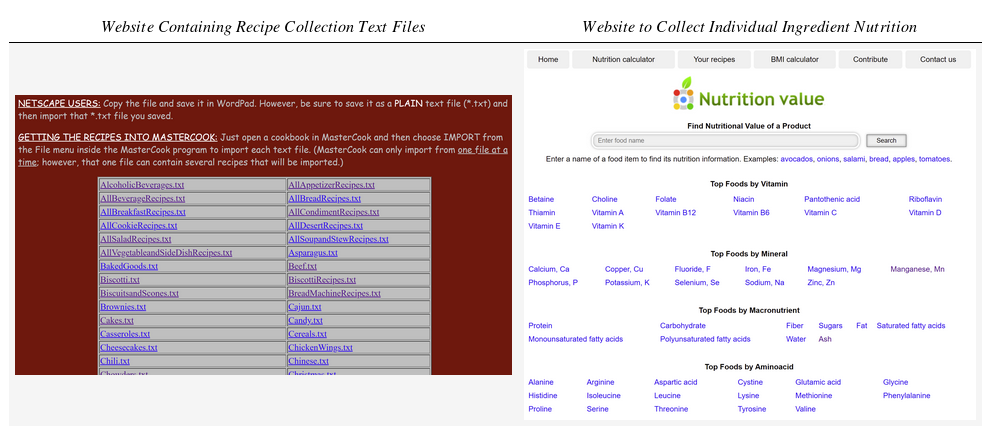
\includegraphics{websites.png}

We will use these two resources to collect the needed information to
create a table that will help us answer our objective questions.

    \hypertarget{validity-of-resources}{%
\paragraph{Validity of Resources}\label{validity-of-resources}}

It is important to note that both of these resources are appropriate for
the question at hand.

The first is valid because it contains recipes that were created by
various users, and offers a variety of recipes. Therefore, the sample of
recipies is well distributed. It is also a suitable source because it
offers a particularly easy way to download the a large number of recipes
with consistant formatting.

The second resource is valid because it pulls its data from the USDA
National Nutrient Database for Standard Reference. It has a broad range
of ingreadients available to search, and is also very detailed in it's
nutritional content breakdown, which makes it suitable for this project.

\hypertarget{table-construction-overview}{%
\subsection{Table Construction
Overview:}\label{table-construction-overview}}

In order to answer the objective questions, we need to create a table
containing the relevent information. We will construct this table after
the following format:

\begin{longtable}[]{@{}lllllll@{}}
\toprule
Category & Recipe & Serving Size & Salt & Sugar & \ldots{} & Ingredient
n\tabularnewline
\midrule
\endhead
Chowders & Clam Chowder & 4 & \ldots{} & \ldots{} & \ldots{} &
\ldots{}\tabularnewline
\bottomrule
\end{longtable}

Each recipe will have an associated category, serving size, and
ingredient columns. Each ingredient column shown here actually
represents a `batch' of many columns that contain: one column for how
much of the ingredient is present, and a column for how much of each
nutritional property (protein content, vitamin content, Calorie count
etc) is contained per 100 grams of that ingredient.

    \hypertarget{data-collection-and-cleaning}{%
\section{Data Collection and
Cleaning:}\label{data-collection-and-cleaning}}

In order to form the desired table, we first need to collect the recipes
and their associated ingredient nutritional information. The process for
this is broken down into two steps: recipe collection and ingredient
information collection.

\hypertarget{recipe-collection-procedure}{%
\subsection{Recipe Collection
Procedure:}\label{recipe-collection-procedure}}

\hypertarget{link-collection}{%
\subsubsection{Link Collection}\label{link-collection}}

In order to collect the information for the recipes, we need to first
scrape all the links that will lead to the text files of each category.
Each link contains a text file that looks like a list of recipes such as
the picture on the left below. The recipies consist of the title,
ingredients, and an explanation portion on how to `make' the recipe. The
portion of each recipe we will be using is just the quantitative
portion, for which an example is given at the right.

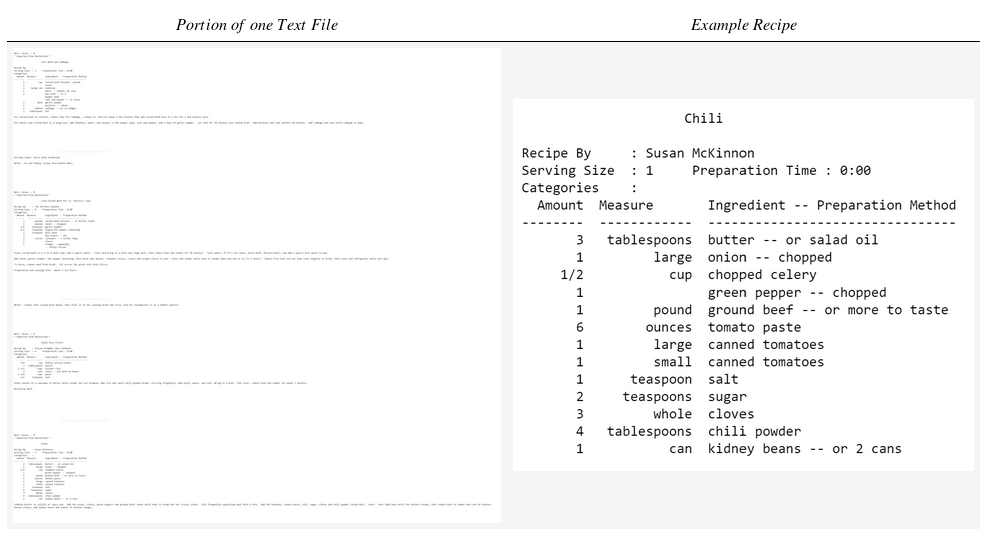
\includegraphics{2textimg.png}

We need to first thus scrape the website of the appropriate links, and
then scrape each link of the list of recipes it contains. Here is some
code that does that:

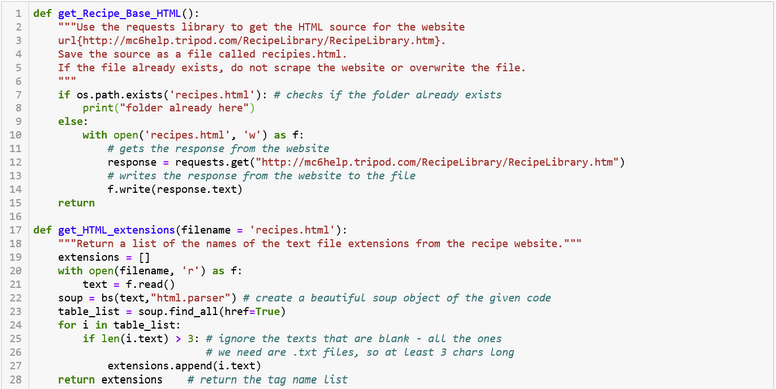
\includegraphics{split1.png}

    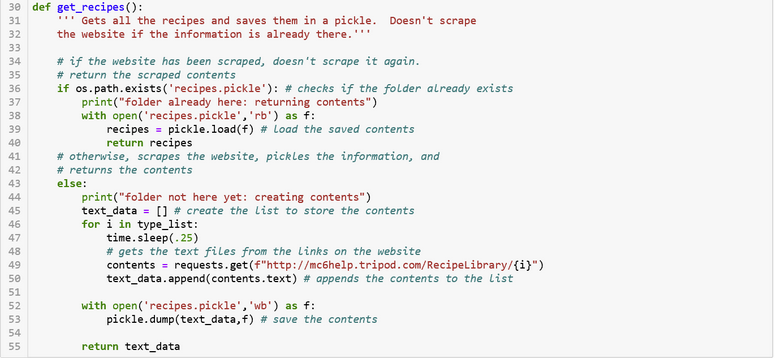
\includegraphics{split2.png}

    \hypertarget{create-recipe-categories}{%
\subsubsection{Create Recipe
Categories}\label{create-recipe-categories}}

We then use the titles of each scraped link to make a list of the
category names.

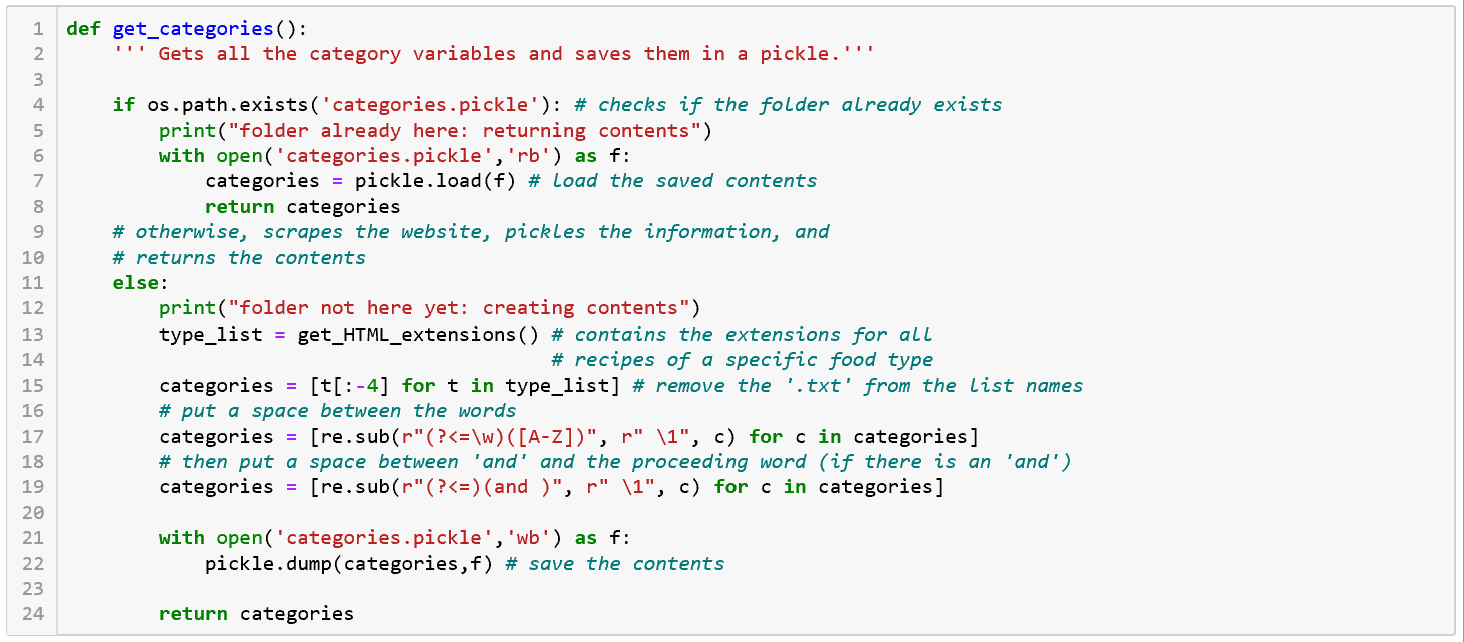
\includegraphics{find_rcategories_code.png}

In all, there are 85 different categories, and they have names such as
`Alcoholic Beverages', `All Appetizer Recipes', `All Beverage Recipes',
`All Bread Recipes', `All Breakfast Recipes', \ldots{}, `Biscuits and
Scones', `Bread Machine Recipes', `Brownies',\ldots{} and many more.

    \hypertarget{separate-individual-recipes}{%
\subsubsection{Separate Individual
Recipes}\label{separate-individual-recipes}}

We then separate each category's single long string of recipes into a
list of strings each containing one recipe. We use Regex to do this in
the following manner:

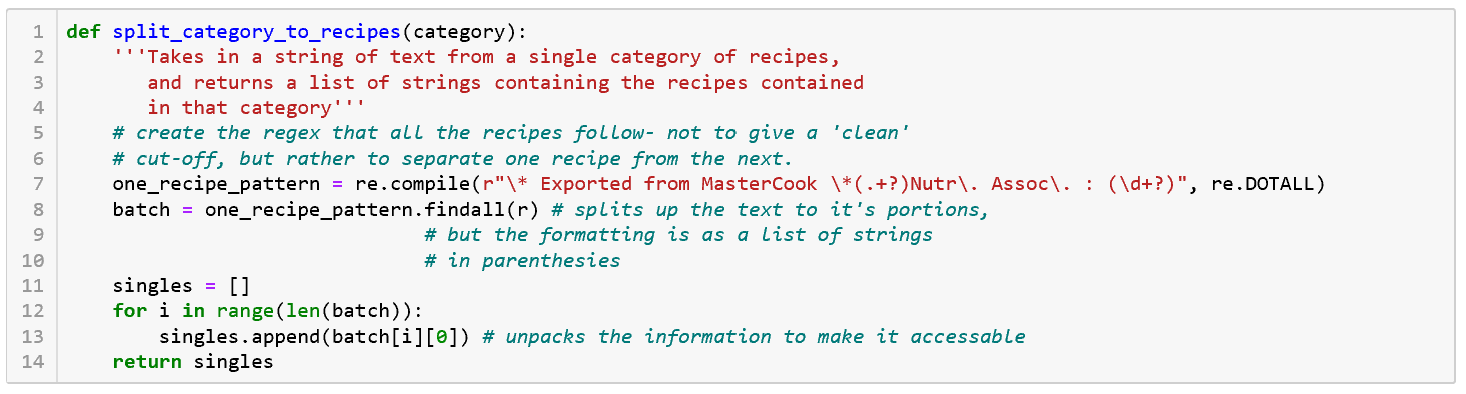
\includegraphics{separate_recipes_code.png}

\hypertarget{get-ingredient-info}{%
\subsubsection{Get Ingredient Info}\label{get-ingredient-info}}

Now we take each recipe, and use Regex to separate out the title,
serving size, and `ingredients batch' (which is a string contianing the
ingredients, their quantities and units of measurement)

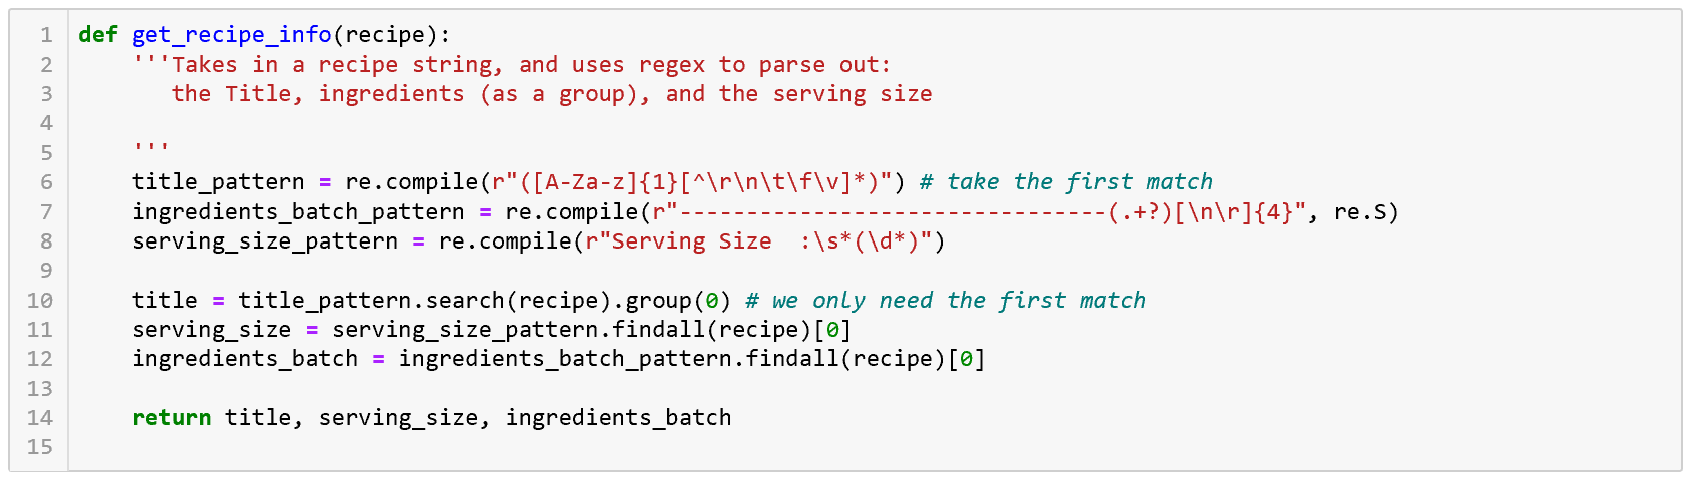
\includegraphics{get_recipe_info_code.png}

    \hypertarget{create-first-basic-table}{%
\subsubsection{Create first basic
table}\label{create-first-basic-table}}

Now we want to create a table that uses the data that we are able to
successfully scrape.

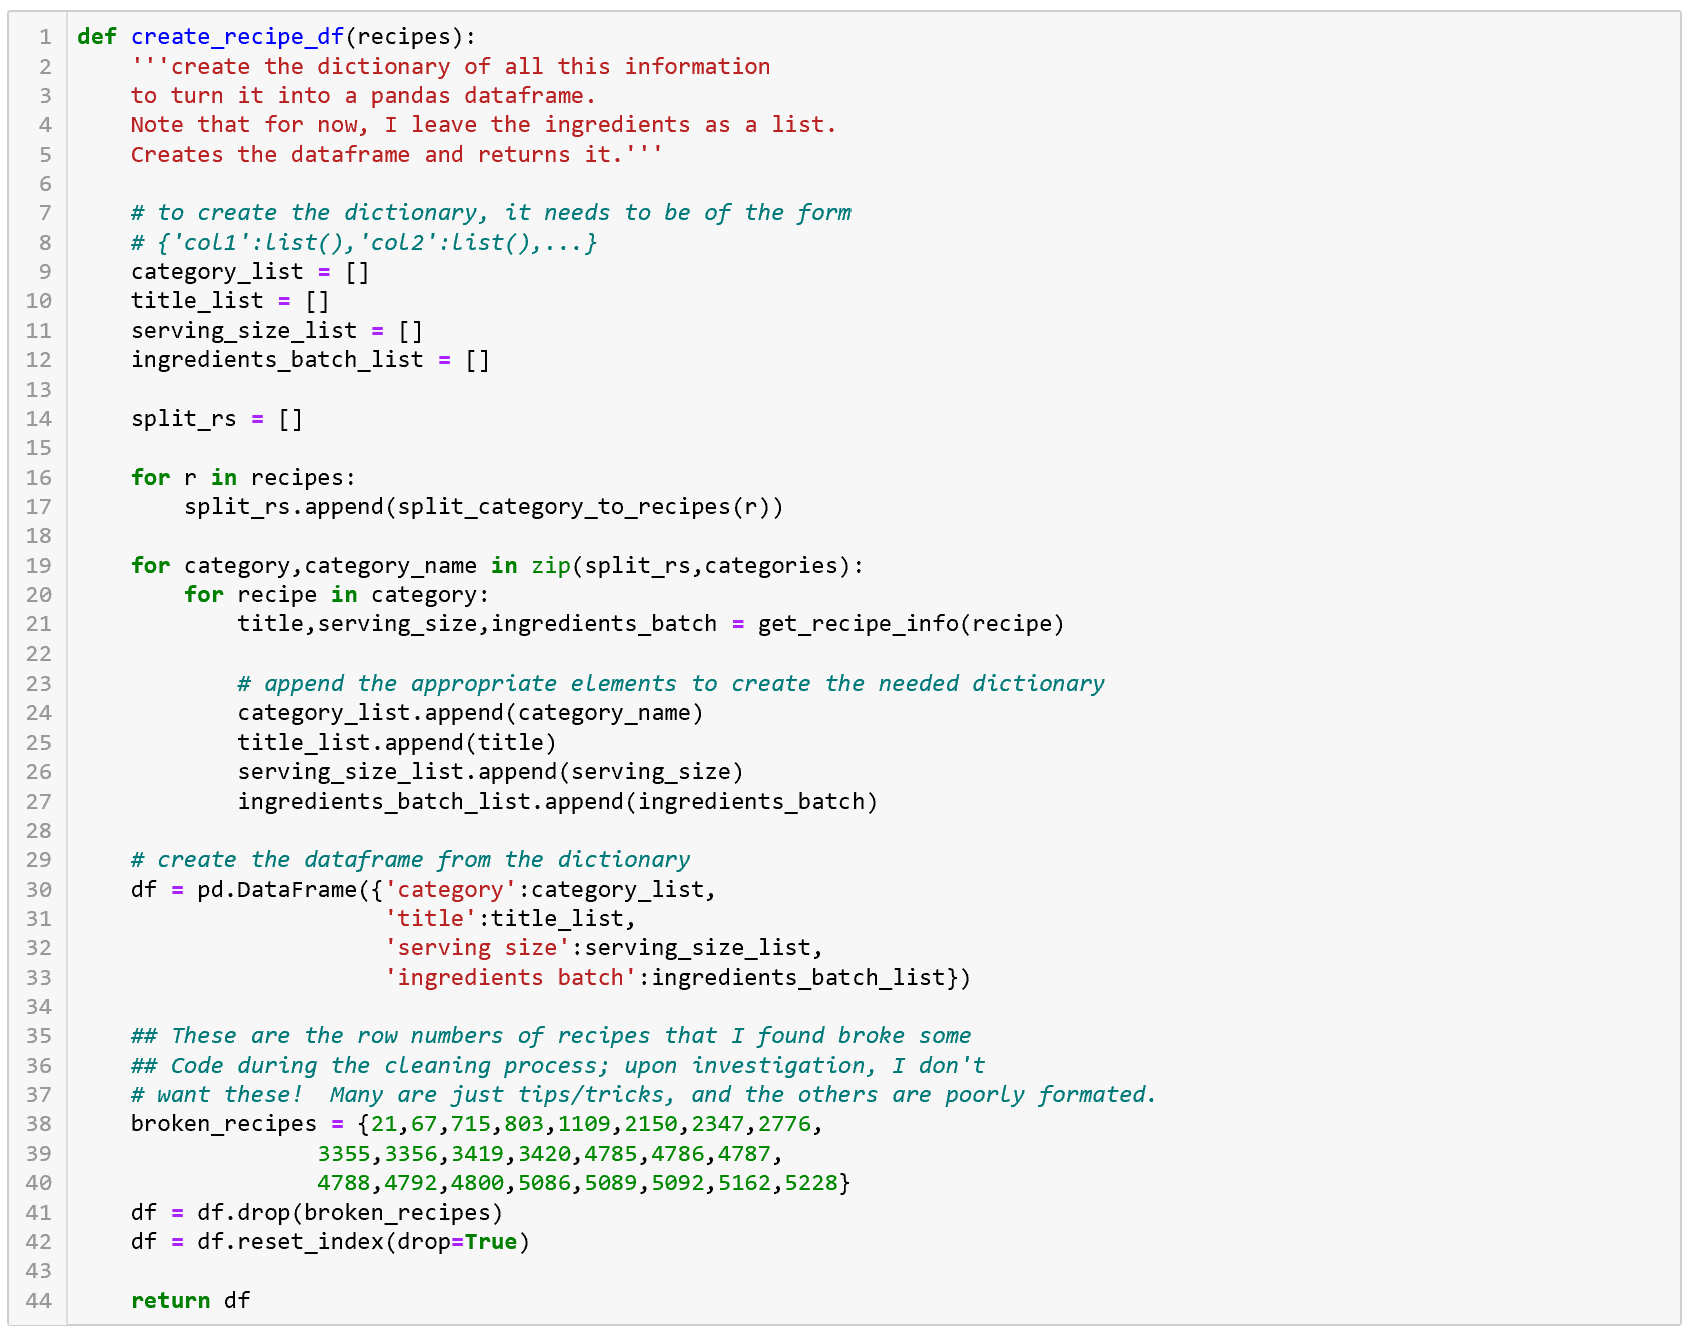
\includegraphics{create_recipe_df_code.png}

Here's the table that we end up with here:

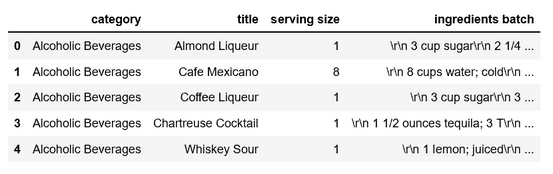
\includegraphics{basic_table_head.png}

\hypertarget{dropping-missformatted-recipes}{%
\subsubsection{Dropping Missformatted
Recipes}\label{dropping-missformatted-recipes}}

Note that we drop some of the recipes because they don't fit the correct
formatting, and there are few enough of them that they don't pose too
much of a loss to the overall effort of creating a table that represents
the nutritional values of various recipes. It was interesting to note
however that the category with the most `erroneous' recipes was that of
`Sourdough bread' - there were multiple instances where people would
give `hints' about how to care for the bread, rather than actually
providing a recipe!

\hypertarget{example-of-poorly-formatted-recipe}{%
\paragraph{\texorpdfstring{\[ Example\ of\ poorly\ formatted\ recipe \]}{ Example\textbackslash{} of\textbackslash{} poorly\textbackslash{} formatted\textbackslash{} recipe }}\label{example-of-poorly-formatted-recipe}}

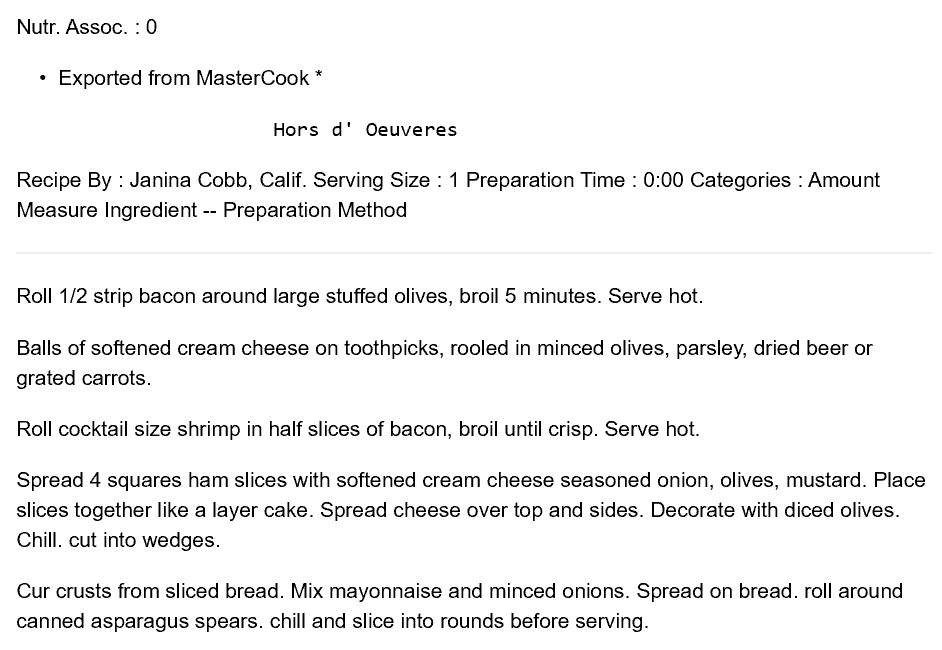
\includegraphics{bad_recipe.png}

    \hypertarget{parsing-the-ingredient-information}{%
\subsubsection{Parsing the Ingredient
Information}\label{parsing-the-ingredient-information}}

We now need to go through the recipe data and separate it out into it's
constituant parts: separate the ingredient name from the quantity from
the unit. Here is a sample of code used to do that:

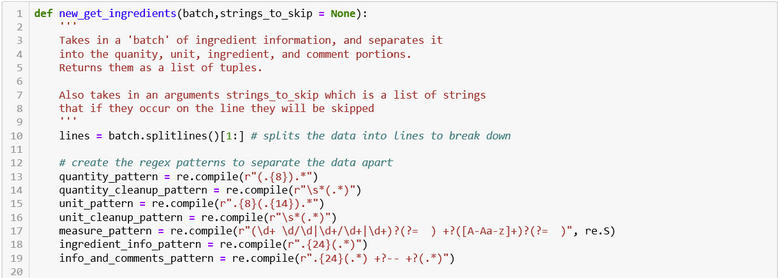
\includegraphics{screen3.png}

    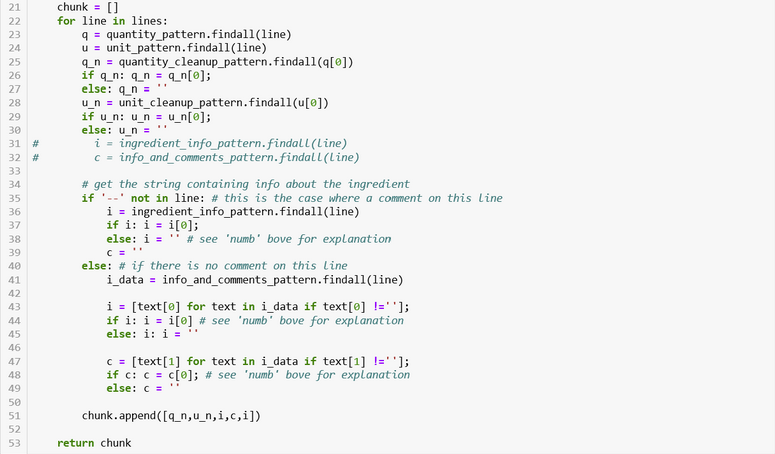
\includegraphics{split4.png}

\hypertarget{normalize-ingreadient-names}{%
\subsubsection{Normalize ingreadient
names}\label{normalize-ingreadient-names}}

Next we need to have a way of normalizing the ingredient names. This is
because many ingredients are presented slightly differently. For
example, brown sugar, dark brown sugar, lightly-packed brown sugar, and
Brn. sugar could all be reasonably categorized into the same ingredient
class: ``brown sugar.''

In order to do this, we first normalized all the ingredients to make
them lowercase.

We then created `class' categories by looking at the most common 200
ingredient types and creating a category for each of them. We selected
the top 200 categories because the 200th most common ingredient is only
used in about 12 of the roughly 5,500 recipes we scraped from, and there
were over 10,000 ingredients total. Thus we decided the tail of
ingredients that were used very little could be cut off, and the
majority of the informational content would still be observed in the
table we are creating.

We ultimately created a dictionary that mapped the raw ingredient name
to the class to which it pertains. (See pertinant Code in the Appendix)

For the classes that did not fit into a category, we put their
information in an `OTHER' class, allowing us to cleanly sort through the
data.

    \hypertarget{create-second-basic-table}{%
\subsubsection{Create Second Basic
Table}\label{create-second-basic-table}}

With the categories created, we can now create the basic layout of our
recipe-ingredients table. The following is the head of this dataframe,
with the ingredients separated out, but the nutritional information of
each ingredient not yet present.

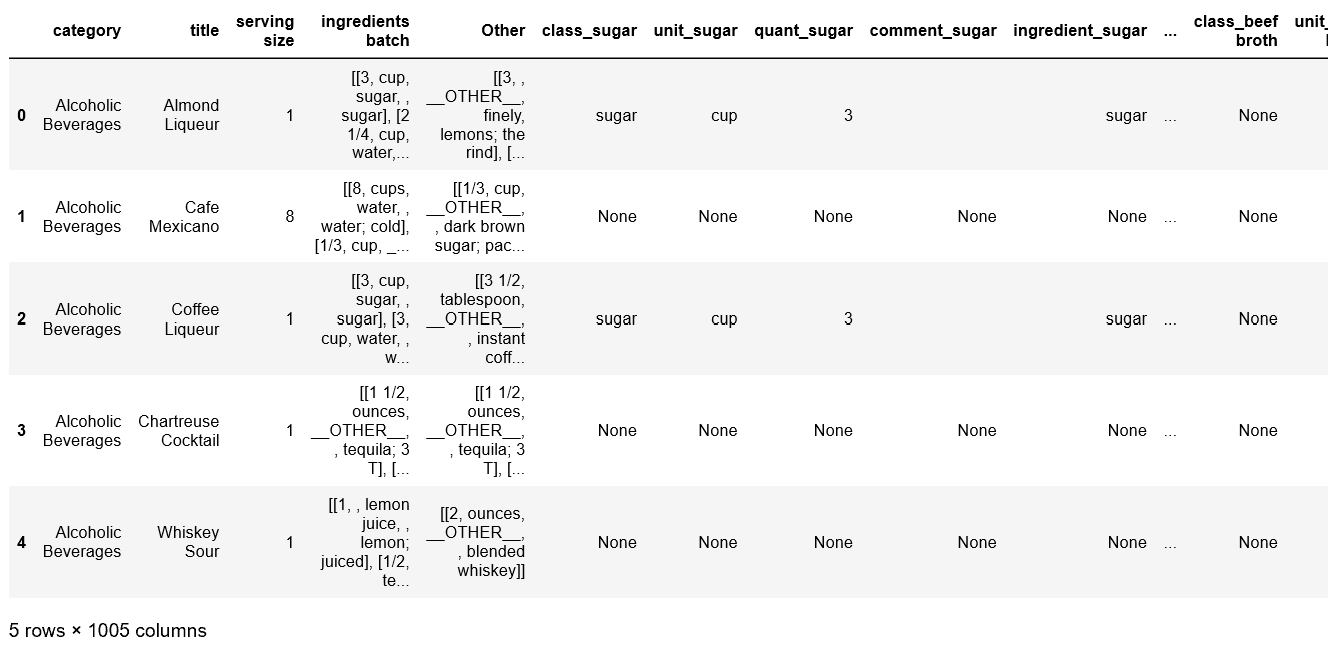
\includegraphics{sorted_dataframe_head.png}

    \hypertarget{ingredient-information-collection-procedure}{%
\subsection{Ingredient Information Collection
Procedure:}\label{ingredient-information-collection-procedure}}

Now that we have the individual ingredients we can start collecting
nutritional data. The site that we used is okay with us using their data
as long as we are not going to sell it.

    The scaper we built for this task searches each ingredient on
nutritionvalue.org and takes the first available 3 links. The reason for
this is that the top link might not be what we are looking for but,
since they are ordered by relevance, it is highly likely to be on the
top three.

Example of query with Oats:

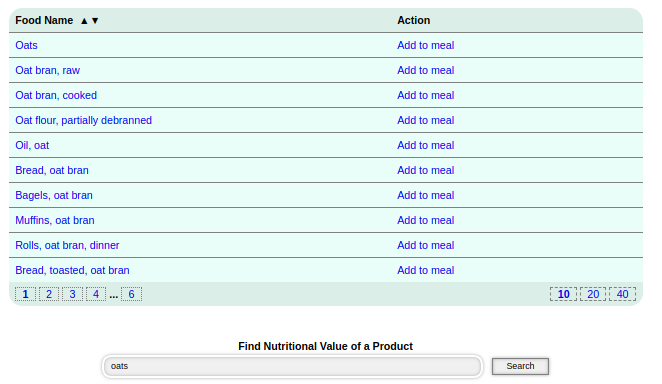
\includegraphics{nutrition_value_query.png}

    These links are collected in a dictionary with the ingredient as its
respective value. The code is able to handle common errors like ``no
results'', ``less than 3 links'', and "can't find search bar.

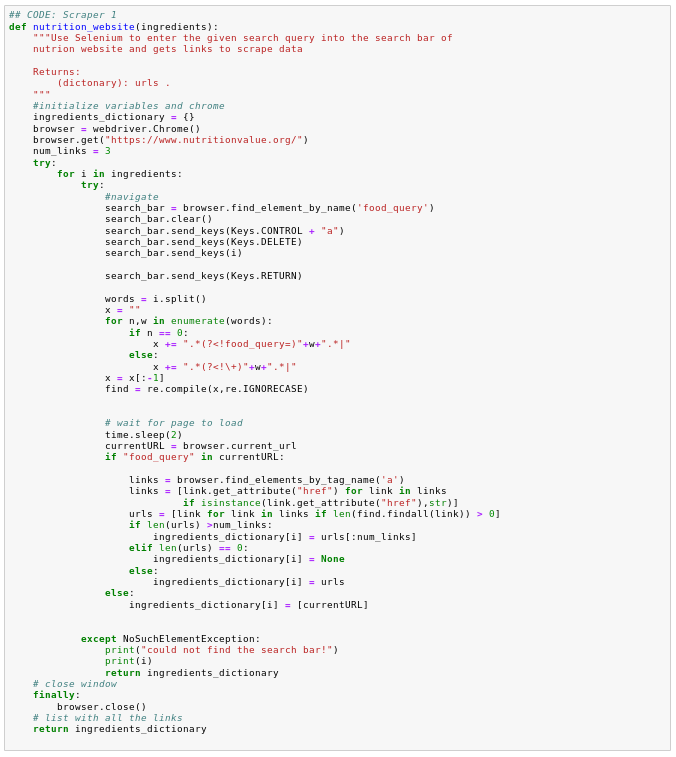
\includegraphics{isaac_code1.png}

    \hypertarget{nutrition-values}{%
\paragraph{Nutrition Values}\label{nutrition-values}}

Now we are ready to get the nutritional value.

Each ingredient link contains tables of nutritonal properties and their
quantities. Here is an example of the content of the link related to
``Oats''.

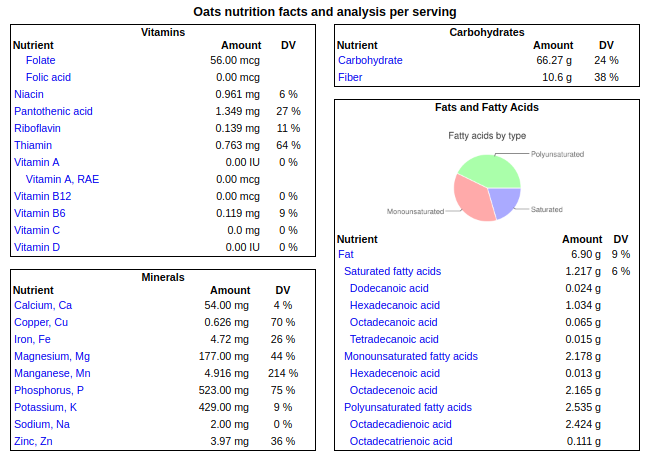
\includegraphics{nutrition_values_oats.png}

    The scaper will go through the dictionary of links and collect the name,
serving size, macronutries (Protein, fat, carbohydrates), micronutrients
(vitamins and minerals), and any other fact on the tables available.

The code prints out any links that cause an error to help minimize the
number of missing ingredients. There were a few links with error but we
inspected them and made sure we weren't losing any important
information. They turned out to be links that were not related to food
but rather other parts of the website that were at times included in our
query.

In order to not abuse the websites information we also added an argument
that skips the search if it has already been pulled.

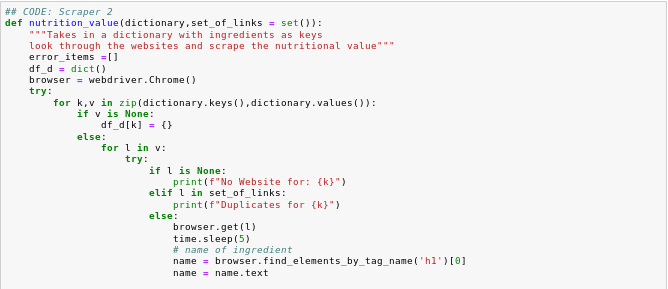
\includegraphics{split5.png}

    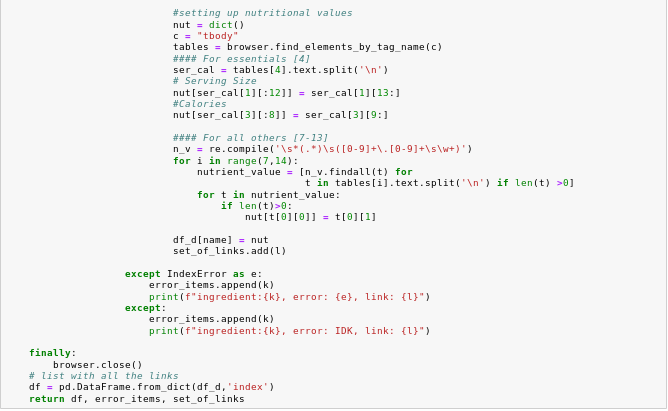
\includegraphics{split6.png}

    \hypertarget{cleaning-nutritional-data}{%
\paragraph{Cleaning Nutritional Data}\label{cleaning-nutritional-data}}

Once we collected the data we analyzed it for errors. There were two
columns that had only one value out of all the ingredients - the number
``18'' and ``adjusted Protein''. For this reason we dropped those
columns.

The rest of the data was cleaned by making all values floats, converting
values to grams (g) and making serving sizes be 1g for all ingredients.

Vitamin A and D were a special case because they were measured in
International Units (IU) so we converted them to grams

Lastly, we engineered a columns for all minerals and vitamins for future
investigation of trends in nutrition - Whether you can get all the
nutrition you need from certain foods or recipes.

This is our nutrtional\_value dataframe

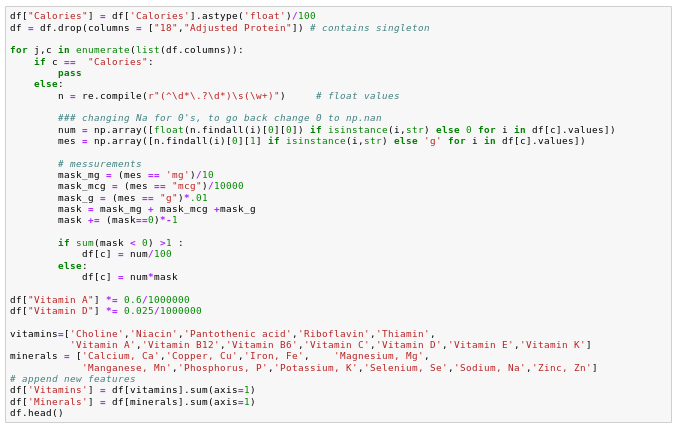
\includegraphics{isaac_code4.png}

    Now that both data sets are clean and contain featured columns, we begin
the merging process to produce a giant sparse dataframe where the rows
are recipies and the columns are ingredient's (ing) nutritional
properties for all ingredients. example:

\begin{longtable}[]{@{}lllllll@{}}
\toprule
recipe & ing1\_calories & ing1\_protein & \ldots{} & ing1\_minerals &
ing2\_calories & \ldots{}\tabularnewline
\midrule
\endhead
\bottomrule
\end{longtable}

In the transition to one data frame we encountered one of our biggest
challenges thus far. We need to sort through the quantities of each
ingredient and convert them to grams. Unfortunately, we have not found a
comprehensive list of food densities online, and the measurements are
not consistent on the recipe website. We have created a temporal
solution that converts abstract measurements into the equivalent in
grams for the most used ingredient and we map words that mean the same
things to a uniform name (ex: tbs, tablesp, TBS -\textgreater{}
tablespoon, See appendix for code).

Small Example of unit converter:

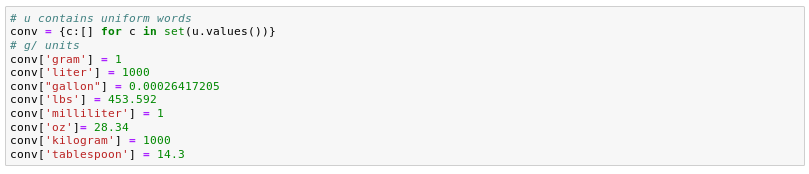
\includegraphics{isaac_code5.png}

    We are continually searching for a solution to the conversion problem.
Nevertheless, We proceed with the analysis so that when an improvement
to this method is found we can get better results.

There are multiple steps to build what we are calling ``Hefty\_df''. For
each recipe we find the ingredients it requires and look up the units
and quantities. For the quantities we built a function that takes in
strings of the form ``1/2 ,5 3/2, None'' and returns its float
equivalent or 1 for None (it represents ``whole''). This ingredient is
found in our ingredients/nutrional value dataframe by the Levenshtein
distance which compares the similarity of words by comparing how many
edits are needed to change one word into the other. For example by
adding or dropping a letter. We then multiply the quantity, unit (using
our unit converter), and the nutritional value of the ingredient and
place them into hefty\_df. Lastly, we sum the values of each property
and enter it into the ``total\_(respective property)'' and repeat the
process (*see apendix for code).

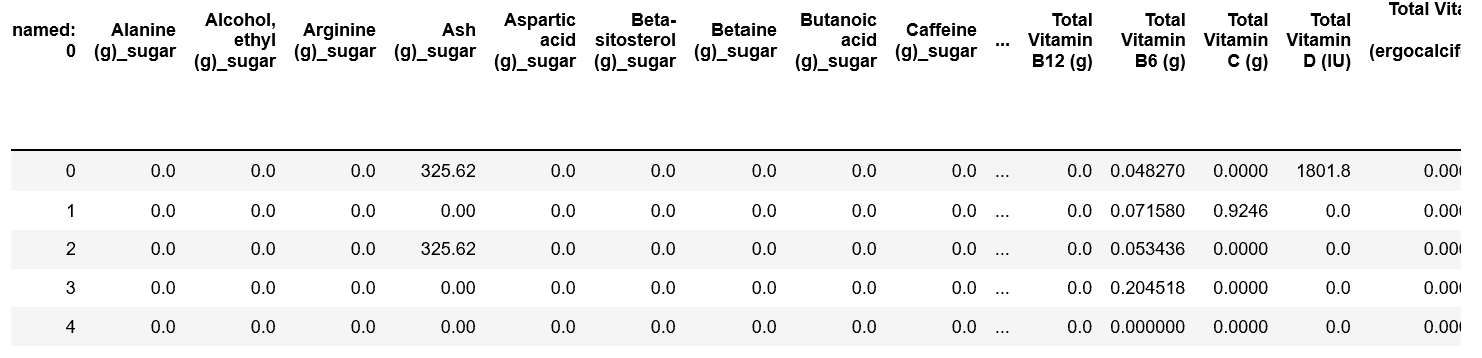
\includegraphics{hefty_head.png}

The reason we built this sparse dataframe is for the intends and
purposes of next semester. We use the columns with the total nutritional
values columns and the ingredients/nutritional value dataframe for our
analyzis.

    \hypertarget{data-visualization-and-analysis}{%
\section{Data Visualization and
Analysis}\label{data-visualization-and-analysis}}

    \begin{itemize}
\tightlist
\item
  PROTEIN
\end{itemize}

    \begin{itemize}
\tightlist
\item
  FAT
\end{itemize}

    There is an important distinction between the different fat values
printed on a produce. Our body needs the good fats (``Polyunsaturated
fatty acids'' and ``Monounsaturated fatty acids'') and could go without
the bad ones (``Saturated fatty acids'' and ``Trans fats''). We wish to
find out how recipe styles vary in their ``good fat to bad fat'' ratio.
It is important to note that these are not true for just one ingredient
(ex: fish, chicke, asparagus,etc.) or a single recipe, rather and
combination of many recipies of that kind.

First we will look at the recipes with high good/bad ratio:

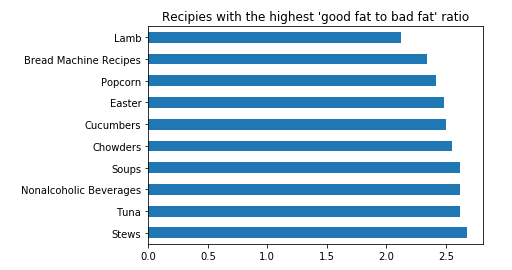
\includegraphics{goodbad1.png}

These are the recipies that would be recommended if someone put the
constraint to have more good fats rather than bad. These results look
resonable since they all tend to have leaner meet and/or recipes that
are considered ``healthier''.

We chose to remove the following categories From the graph above: -
Alchoholic beverage - Most of the ingredients are not well represented
since they are too specific and were put in the ``other'' ingredients
pile - Jam - Likely there are low leves of fat which would make the
ratio extreme depending on one or two recipes - Dog Buiscuits - The
reader can know that they are good for their dog

Likewise, you might want to know which recipies to abstain from
making/eating to stay healthy. The following figure shows the lowest
ratios of good to bad fat.

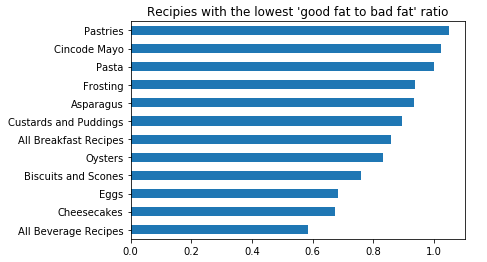
\includegraphics{goodbad2.png}

Once again we have values that we expect like cake, pasta, and breakfast
foods. Asparagus is on there because it is often cooked with butter,
cheese or oils.

    \begin{itemize}
\tightlist
\item
  Vitamins and Minerals
\end{itemize}

Last question we would like to address is whether there is any
correlation between protein, vitamins, and minerals in our list of
ingredients. If so then we know that choosing one high nutritious
ingredient will provide a balance more balance to your diet.

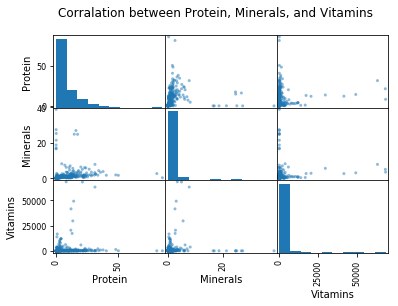
\includegraphics{corr_m.png}

The highest correlation is between protein and Minerals which makes
sense since there is iron in meat, and the lowest is between vitamins
and minerals - Probably the reason they are sold seperately as
supplements.

    \hypertarget{apendix}{%
\section{Apendix}\label{apendix}}

    \hypertarget{code-for-hefty-dataframe}{%
\subsubsection{Code for hefty
DataFrame}\label{code-for-hefty-dataframe}}

    \begin{Verbatim}[commandchars=\\\{\}]
{\color{incolor}In [{\color{incolor} }]:} \PY{c+c1}{\PYZsh{} changing units by hand (only first time seen)}
        \PY{n}{u} \PY{o}{=} \PY{n+nb}{dict}\PY{p}{(}\PY{p}{)}
        \PY{k}{for} \PY{n}{i}\PY{p}{,}\PY{n}{rec} \PY{o+ow}{in} \PY{n+nb}{enumerate}\PY{p}{(}\PY{n}{neal\PYZus{}df}\PY{p}{[}\PY{n}{mask}\PY{p}{]}\PY{o}{.}\PY{n}{values}\PY{p}{)}\PY{p}{:}
            \PY{k}{for} \PY{n}{j}\PY{p}{,}\PY{n}{mes} \PY{o+ow}{in} \PY{n+nb}{enumerate}\PY{p}{(}\PY{n}{rec}\PY{p}{)}\PY{p}{:}
                \PY{k}{if} \PY{n}{mes} \PY{o+ow}{in} \PY{n}{u}\PY{p}{:}
                    \PY{k}{pass}
                \PY{k}{else}\PY{p}{:}
                    \PY{n+nb}{print}\PY{p}{(}\PY{n}{neal\PYZus{}df}\PY{p}{[}\PY{n}{mask}\PY{p}{]}\PY{o}{.}\PY{n}{columns}\PY{p}{[}\PY{n}{j}\PY{p}{]}\PY{p}{)}
                    \PY{n+nb}{print}\PY{p}{(}\PY{n}{mes}\PY{p}{)}
                    \PY{n}{u}\PY{p}{[}\PY{n}{mes}\PY{p}{]} \PY{o}{=} \PY{n+nb}{input}\PY{p}{(}\PY{p}{)}
                    \PY{n+nb}{print}\PY{p}{(}\PY{p}{)}
\end{Verbatim}


    \begin{Verbatim}[commandchars=\\\{\}]
{\color{incolor}In [{\color{incolor} }]:} \PY{c+c1}{\PYZsh{} Unit Conversion dictionary}
        \PY{c+c1}{\PYZsh{} g/ units}
        \PY{n}{conv}\PY{p}{[}\PY{l+s+s1}{\PYZsq{}}\PY{l+s+s1}{gram}\PY{l+s+s1}{\PYZsq{}}\PY{p}{]} \PY{o}{=} \PY{l+m+mi}{1}
        \PY{n}{conv}\PY{p}{[}\PY{l+s+s1}{\PYZsq{}}\PY{l+s+s1}{liter}\PY{l+s+s1}{\PYZsq{}}\PY{p}{]} \PY{o}{=} \PY{l+m+mi}{1000}
        \PY{n}{conv}\PY{p}{[}\PY{l+s+s2}{\PYZdq{}}\PY{l+s+s2}{gallon}\PY{l+s+s2}{\PYZdq{}}\PY{p}{]} \PY{o}{=} \PY{l+m+mf}{0.00026417205}
        \PY{n}{conv}\PY{p}{[}\PY{l+s+s1}{\PYZsq{}}\PY{l+s+s1}{lbs}\PY{l+s+s1}{\PYZsq{}}\PY{p}{]} \PY{o}{=} \PY{l+m+mf}{453.592}
        \PY{n}{conv}\PY{p}{[}\PY{l+s+s1}{\PYZsq{}}\PY{l+s+s1}{milliliter}\PY{l+s+s1}{\PYZsq{}}\PY{p}{]} \PY{o}{=} \PY{l+m+mi}{1}
        \PY{n}{conv}\PY{p}{[}\PY{l+s+s1}{\PYZsq{}}\PY{l+s+s1}{oz}\PY{l+s+s1}{\PYZsq{}}\PY{p}{]}\PY{o}{=} \PY{l+m+mf}{28.34}
        \PY{n}{conv}\PY{p}{[}\PY{l+s+s1}{\PYZsq{}}\PY{l+s+s1}{kilogram}\PY{l+s+s1}{\PYZsq{}}\PY{p}{]} \PY{o}{=} \PY{l+m+mi}{1000}
        \PY{n}{conv}\PY{p}{[}\PY{l+s+s1}{\PYZsq{}}\PY{l+s+s1}{tablespoon}\PY{l+s+s1}{\PYZsq{}}\PY{p}{]} \PY{o}{=} \PY{l+m+mf}{14.3}
        \PY{n}{conv}\PY{p}{[}\PY{l+s+s1}{\PYZsq{}}\PY{l+s+s1}{teaspoon}\PY{l+s+s1}{\PYZsq{}}\PY{p}{]} \PY{o}{=} \PY{l+m+mf}{4.77}
        \PY{n}{conv}\PY{p}{[}\PY{l+s+s2}{\PYZdq{}}\PY{l+s+s2}{cup}\PY{l+s+s2}{\PYZdq{}}\PY{p}{]} \PY{o}{=} \PY{l+m+mi}{201}
        \PY{n}{conv}\PY{p}{[}\PY{l+s+s2}{\PYZdq{}}\PY{l+s+s2}{ear}\PY{l+s+s2}{\PYZdq{}}\PY{p}{]} \PY{o}{=} \PY{l+m+mi}{92}
        \PY{n}{conv}\PY{p}{[}\PY{l+s+s1}{\PYZsq{}}\PY{l+s+s1}{clove}\PY{l+s+s1}{\PYZsq{}}\PY{p}{]} \PY{o}{=} \PY{l+m+mi}{7}
        \PY{n}{conv}\PY{p}{[}\PY{l+s+s1}{\PYZsq{}}\PY{l+s+s1}{pinch}\PY{l+s+s1}{\PYZsq{}}\PY{p}{]} \PY{o}{=} \PY{l+m+mf}{0.36}
        \PY{n}{conv}\PY{p}{[}\PY{l+s+s1}{\PYZsq{}}\PY{l+s+s1}{quart}\PY{l+s+s1}{\PYZsq{}}\PY{p}{]} \PY{o}{=} \PY{l+m+mf}{946.353}
        \PY{n}{conv}\PY{p}{[}\PY{l+s+s1}{\PYZsq{}}\PY{l+s+s1}{pint}\PY{l+s+s1}{\PYZsq{}}\PY{p}{]} \PY{o}{=} \PY{l+m+mf}{473.176}
        \PY{n}{conv}\PY{p}{[}\PY{l+s+s1}{\PYZsq{}}\PY{l+s+s1}{envelope}\PY{l+s+s1}{\PYZsq{}}\PY{p}{]} \PY{o}{=} \PY{l+m+mf}{7.085}
        \PY{n}{conv}\PY{p}{[}\PY{l+s+s1}{\PYZsq{}}\PY{l+s+s1}{None}\PY{l+s+s1}{\PYZsq{}}\PY{p}{]} \PY{o}{=} \PY{l+m+mi}{0}
        \PY{n}{conv}\PY{p}{[}\PY{l+s+s1}{\PYZsq{}}\PY{l+s+s1}{dash}\PY{l+s+s1}{\PYZsq{}}\PY{p}{]} \PY{o}{=} \PY{l+m+mf}{0.72}
        \PY{n}{conv}\PY{p}{[}\PY{l+s+s1}{\PYZsq{}}\PY{l+s+s1}{head}\PY{l+s+s1}{\PYZsq{}}\PY{p}{]} \PY{o}{=} \PY{l+m+mi}{539}
        \PY{n}{conv}\PY{p}{[}\PY{l+s+s1}{\PYZsq{}}\PY{l+s+s1}{stick}\PY{l+s+s1}{\PYZsq{}}\PY{p}{]} \PY{o}{=} \PY{l+m+mi}{113}
        \PY{n}{conv}\PY{p}{[}\PY{l+s+s1}{\PYZsq{}}\PY{l+s+s1}{package}\PY{l+s+s1}{\PYZsq{}}\PY{p}{]} \PY{o}{=} \PY{l+m+mf}{7.085}
        \PY{n}{conv}\PY{p}{[}\PY{l+s+s1}{\PYZsq{}}\PY{l+s+s1}{small}\PY{l+s+s1}{\PYZsq{}}\PY{p}{]} \PY{o}{=} \PY{l+m+mi}{75}
        \PY{n}{conv}\PY{p}{[}\PY{l+s+s1}{\PYZsq{}}\PY{l+s+s1}{medium}\PY{l+s+s1}{\PYZsq{}}\PY{p}{]} \PY{o}{=} \PY{l+m+mi}{150}
        \PY{n}{conv}\PY{p}{[}\PY{l+s+s1}{\PYZsq{}}\PY{l+s+s1}{large}\PY{l+s+s1}{\PYZsq{}}\PY{p}{]} \PY{o}{=} \PY{l+m+mi}{225}
        \PY{n}{conv}\PY{p}{[}\PY{l+s+s1}{\PYZsq{}}\PY{l+s+s1}{stalk}\PY{l+s+s1}{\PYZsq{}}\PY{p}{]} \PY{o}{=} \PY{l+m+mi}{50}
        \PY{n}{conv}\PY{p}{[}\PY{l+s+s1}{\PYZsq{}}\PY{l+s+s1}{strip}\PY{l+s+s1}{\PYZsq{}}\PY{p}{]} \PY{o}{=} \PY{l+m+mi}{10}
        \PY{n}{conv}\PY{p}{[}\PY{l+s+s1}{\PYZsq{}}\PY{l+s+s1}{square}\PY{l+s+s1}{\PYZsq{}}\PY{p}{]} \PY{o}{=} \PY{l+m+mi}{13}
        \PY{n}{conv}\PY{p}{[}\PY{l+s+s1}{\PYZsq{}}\PY{l+s+s1}{square}\PY{l+s+s1}{\PYZsq{}}\PY{p}{]} \PY{o}{=} \PY{l+m+mf}{56.7}
        \PY{n}{conv}\PY{p}{[}\PY{l+s+s1}{\PYZsq{}}\PY{l+s+s1}{box}\PY{l+s+s1}{\PYZsq{}}\PY{p}{]} \PY{o}{=} \PY{l+m+mf}{382.59}
        \PY{n}{conv}\PY{p}{[}\PY{l+s+s1}{\PYZsq{}}\PY{l+s+s1}{whole}\PY{l+s+s1}{\PYZsq{}}\PY{p}{]} \PY{o}{=} \PY{l+m+mi}{100}
        \PY{n}{conv}\PY{p}{[}\PY{l+s+s1}{\PYZsq{}}\PY{l+s+s1}{bag}\PY{l+s+s1}{\PYZsq{}}\PY{p}{]} \PY{o}{=} \PY{l+m+mf}{453.59}
        \PY{n}{conv}\PY{p}{[}\PY{l+s+s1}{\PYZsq{}}\PY{l+s+s1}{sprig}\PY{l+s+s1}{\PYZsq{}}\PY{p}{]} \PY{o}{=} \PY{l+m+mi}{30}
        \PY{n}{conv}\PY{p}{[}\PY{l+s+s1}{\PYZsq{}}\PY{l+s+s1}{bulb}\PY{l+s+s1}{\PYZsq{}}\PY{p}{]} \PY{o}{=} \PY{l+m+mi}{30}
        \PY{n}{conv}\PY{p}{[}\PY{l+s+s1}{\PYZsq{}}\PY{l+s+s1}{slice}\PY{l+s+s1}{\PYZsq{}}\PY{p}{]} \PY{o}{=} \PY{l+m+mi}{5}
        \PY{n}{conv}\PY{p}{[}\PY{l+s+s1}{\PYZsq{}}\PY{l+s+s1}{bunch}\PY{l+s+s1}{\PYZsq{}}\PY{p}{]} \PY{o}{=} \PY{l+m+mi}{120}
        \PY{n}{conv}\PY{p}{[}\PY{l+s+s1}{\PYZsq{}}\PY{l+s+s1}{part}\PY{l+s+s1}{\PYZsq{}}\PY{p}{]} \PY{o}{=} \PY{l+m+mi}{1}
        \PY{n}{conv}\PY{p}{[}\PY{l+s+s1}{\PYZsq{}}\PY{l+s+s1}{cube}\PY{l+s+s1}{\PYZsq{}}\PY{p}{]} \PY{o}{=} \PY{l+m+mi}{57}
\end{Verbatim}


    \begin{Verbatim}[commandchars=\\\{\}]
{\color{incolor}In [{\color{incolor} }]:} \PY{c+c1}{\PYZsh{} gets mask for ingredients}
        \PY{n}{col} \PY{o}{=} \PY{n+nb}{list}\PY{p}{(}\PY{n}{neal\PYZus{}df}\PY{o}{.}\PY{n}{columns}\PY{p}{)} 
        \PY{n}{mask\PYZus{}class} \PY{o}{=} \PY{n}{np}\PY{o}{.}\PY{n}{array}\PY{p}{(}\PY{p}{[}\PY{n}{i} \PY{k}{for} \PY{n}{i} \PY{o+ow}{in} \PY{n}{col} \PY{k}{if} \PY{n}{i}\PY{p}{[}\PY{p}{:}\PY{l+m+mi}{6}\PY{p}{]} \PY{o}{==} \PY{l+s+s2}{\PYZdq{}}\PY{l+s+s2}{class\PYZus{}}\PY{l+s+s2}{\PYZdq{}}\PY{p}{]}\PY{p}{)}
\end{Verbatim}


    \begin{Verbatim}[commandchars=\\\{\}]
{\color{incolor}In [{\color{incolor} }]:} \PY{c+c1}{\PYZsh{} create the columns for Hefty}
        \PY{n}{hefty\PYZus{}columns} \PY{o}{=} \PY{p}{[}\PY{n}{nut\PYZus{}element}\PY{o}{+}\PY{l+s+s2}{\PYZdq{}}\PY{l+s+s2}{\PYZus{}}\PY{l+s+s2}{\PYZdq{}}\PY{o}{+}\PY{n}{category}\PY{p}{[}\PY{l+m+mi}{6}\PY{p}{:}\PY{p}{]} \PY{k}{for} \PY{n}{category} \PY{o+ow}{in} \PY{n}{mask\PYZus{}class} \PY{k}{for} \PY{n}{nut\PYZus{}element} \PY{o+ow}{in} \PY{n}{df}\PY{o}{.}\PY{n}{columns}\PY{p}{]}
        \PY{n}{hefty\PYZus{}columns} \PY{o}{+}\PY{o}{=} \PY{p}{[}\PY{l+s+s2}{\PYZdq{}}\PY{l+s+s2}{Total }\PY{l+s+s2}{\PYZdq{}}\PY{o}{+} \PY{n}{nut\PYZus{}element} \PY{k}{for} \PY{n}{nut\PYZus{}element} \PY{o+ow}{in} \PY{n}{df}\PY{o}{.}\PY{n}{columns}\PY{p}{]}
\end{Verbatim}


    \begin{Verbatim}[commandchars=\\\{\}]
{\color{incolor}In [{\color{incolor} }]:} \PY{c+c1}{\PYZsh{} Turning strings to floats}
        \PY{k}{def} \PY{n+nf}{st\PYZus{}to\PYZus{}fl}\PY{p}{(}\PY{n}{s}\PY{p}{)}\PY{p}{:}
            \PY{k}{try}\PY{p}{:}
                \PY{c+c1}{\PYZsh{} This implied \PYZdq{}Whole\PYZdq{}}
                \PY{k}{if} \PY{n}{s} \PY{o+ow}{is} \PY{k+kc}{None}\PY{p}{:}
                    \PY{k}{return} \PY{l+m+mi}{1}
                \PY{c+c1}{\PYZsh{} other wise make it float}
                \PY{k}{return} \PY{n+nb}{float}\PY{p}{(}\PY{n}{s}\PY{p}{)}
            \PY{k}{except} \PY{n+ne}{ValueError}\PY{p}{:}
                \PY{c+c1}{\PYZsh{}if error do this}
                \PY{k}{return} \PY{n+nb}{float}\PY{p}{(}\PY{n+nb}{sum}\PY{p}{(}\PY{n}{Fraction}\PY{p}{(}\PY{n}{c}\PY{p}{)} \PY{k}{for} \PY{n}{c} \PY{o+ow}{in} \PY{n}{s}\PY{o}{.}\PY{n}{split}\PY{p}{(}\PY{p}{)}\PY{p}{)}\PY{p}{)}
\end{Verbatim}


    \begin{Verbatim}[commandchars=\\\{\}]
{\color{incolor}In [{\color{incolor} }]:} \PY{c+c1}{\PYZsh{} building hefty}
        \PY{n}{hefty\PYZus{}df} \PY{o}{=} \PY{n}{pd}\PY{o}{.}\PY{n}{DataFrame}\PY{p}{(}\PY{n}{columns}\PY{o}{=}\PY{n}{hefty\PYZus{}columns}\PY{p}{)}
        \PY{n}{num\PYZus{}recipies} \PY{o}{=} \PY{n+nb}{len}\PY{p}{(}\PY{n+nb}{list}\PY{p}{(}\PY{n}{neal\PYZus{}df}\PY{o}{.}\PY{n}{index}\PY{p}{)}\PY{p}{)}
        
        \PY{c+c1}{\PYZsh{} for each recipe}
        \PY{k}{for} \PY{n}{num}\PY{p}{,} \PY{n}{recipe} \PY{o+ow}{in} \PY{n+nb}{enumerate}\PY{p}{(}\PY{n}{neal\PYZus{}df}\PY{o}{.}\PY{n}{index}\PY{p}{)}\PY{p}{:}
            \PY{c+c1}{\PYZsh{} get all the entries and get the values that are not None}
            \PY{n}{r} \PY{o}{=} \PY{n}{neal\PYZus{}df}\PY{o}{.}\PY{n}{iloc}\PY{p}{[}\PY{n}{recipe}\PY{p}{]}
            \PY{n}{r\PYZus{}contents} \PY{o}{=} \PY{n}{r}\PY{p}{[}\PY{n}{mask\PYZus{}class}\PY{p}{]}\PY{o}{.}\PY{n}{values} \PY{o}{!=} \PY{k+kc}{None} \PY{c+c1}{\PYZsh{} mask}
            
            \PY{c+c1}{\PYZsh{}get the values where it wasn\PYZsq{}t none and inicialize the row}
            \PY{n}{ingredients} \PY{o}{=} \PY{n}{r}\PY{p}{[}\PY{n}{mask\PYZus{}class}\PY{p}{]}\PY{p}{[}\PY{n}{r\PYZus{}contents}\PY{p}{]}\PY{o}{.}\PY{n}{values}
            \PY{n}{hefty\PYZus{}df}\PY{o}{.}\PY{n}{loc}\PY{p}{[}\PY{n+nb}{len}\PY{p}{(}\PY{n}{hefty\PYZus{}df}\PY{p}{)}\PY{p}{]} \PY{o}{=} \PY{l+m+mi}{0}
            
            \PY{c+c1}{\PYZsh{}progress bar}
            \PY{k}{if} \PY{n}{num}\PY{o}{\PYZpc{}} \PY{l+m+mi}{200} \PY{o}{==} \PY{l+m+mi}{0}\PY{p}{:}
                \PY{n+nb}{print}\PY{p}{(}\PY{n}{f}\PY{l+s+s2}{\PYZdq{}}\PY{l+s+s2}{\PYZob{}}\PY{l+s+s2}{num/num\PYZus{}recipies\PYZcb{}}\PY{l+s+s2}{\PYZpc{}}\PY{l+s+s2}{\PYZdq{}}\PY{p}{)}
                
            \PY{c+c1}{\PYZsh{} for each ingredient in the recipe}
            \PY{k}{for} \PY{n}{ing} \PY{o+ow}{in} \PY{n}{ingredients}\PY{p}{:}
                \PY{c+c1}{\PYZsh{} change the quantity to float and convert units to grams}
                \PY{n}{quantity} \PY{o}{=} \PY{n}{st\PYZus{}to\PYZus{}fl}\PY{p}{(}\PY{n}{r}\PY{p}{[}\PY{l+s+s1}{\PYZsq{}}\PY{l+s+s1}{quant\PYZus{}}\PY{l+s+s1}{\PYZsq{}} \PY{o}{+} \PY{n}{ing}\PY{p}{]}\PY{p}{)}
                \PY{n}{unit\PYZus{}factor} \PY{o}{=} \PY{n}{conv}\PY{p}{[}\PY{n}{r}\PY{p}{[}\PY{l+s+s1}{\PYZsq{}}\PY{l+s+s1}{unit\PYZus{}}\PY{l+s+s1}{\PYZsq{}} \PY{o}{+} \PY{n}{ing}\PY{p}{]}\PY{p}{]}
                \PY{n}{conversion} \PY{o}{=} \PY{n}{quantity}\PY{o}{*}\PY{n}{unit\PYZus{}factor}  
                
                \PY{c+c1}{\PYZsh{}find the most similar ingredient in the nutrition data frame}
                \PY{n}{most\PYZus{}similar\PYZus{}ing} \PY{o}{=} \PY{n}{process}\PY{o}{.}\PY{n}{extractOne}\PY{p}{(}\PY{n}{ing}\PY{p}{,}\PY{n}{df}\PY{o}{.}\PY{n}{index}\PY{p}{)}\PY{p}{[}\PY{l+m+mi}{0}\PY{p}{]}
                
                \PY{c+c1}{\PYZsh{} match the columns of hefty with the ingredient}
                \PY{n}{col} \PY{o}{=} \PY{n+nb}{list}\PY{p}{(}\PY{n}{hefty\PYZus{}df}\PY{o}{.}\PY{n}{columns}\PY{p}{)} 
                \PY{n}{hefty\PYZus{}mask} \PY{o}{=} \PY{n}{np}\PY{o}{.}\PY{n}{array}\PY{p}{(}\PY{p}{[}\PY{n}{i} \PY{k}{for} \PY{n}{i} \PY{o+ow}{in} \PY{n}{col} \PY{k}{if} \PY{n}{i}\PY{p}{[}\PY{o}{\PYZhy{}}\PY{p}{(}\PY{n+nb}{len}\PY{p}{(}\PY{n}{ing}\PY{p}{)}\PY{o}{+}\PY{l+m+mi}{1}\PY{p}{)}\PY{p}{:}\PY{p}{]} \PY{o}{==} \PY{l+s+s2}{\PYZdq{}}\PY{l+s+s2}{\PYZus{}}\PY{l+s+s2}{\PYZdq{}}\PY{o}{+}\PY{n}{ing}\PY{p}{]}\PY{p}{)}
                
                \PY{c+c1}{\PYZsh{} for each column with the ingredient mutiply nutrition value by conversion}
                \PY{c+c1}{\PYZsh{} and add to total column}
                \PY{k}{for} \PY{n}{m}\PY{p}{,}\PY{n}{i}\PY{p}{,}\PY{n}{c} \PY{o+ow}{in} \PY{n+nb}{zip}\PY{p}{(}\PY{n}{hefty\PYZus{}mask}\PY{p}{,} \PY{n}{df}\PY{o}{.}\PY{n}{loc}\PY{p}{[}\PY{n}{most\PYZus{}similar\PYZus{}ing}\PY{p}{]}\PY{o}{.}\PY{n}{values}\PY{p}{,}\PY{n}{df}\PY{o}{.}\PY{n}{columns}\PY{p}{)}\PY{p}{:}
                    \PY{n}{value} \PY{o}{=} \PY{n}{i}\PY{o}{*}\PY{n}{conversion}
                    \PY{n}{hefty\PYZus{}df}\PY{o}{.}\PY{n}{loc}\PY{p}{[}\PY{n}{num}\PY{p}{]}\PY{p}{[}\PY{n}{m}\PY{p}{]} \PY{o}{=} \PY{n}{value}
                    \PY{n}{hefty\PYZus{}df}\PY{o}{.}\PY{n}{loc}\PY{p}{[}\PY{n}{num}\PY{p}{]}\PY{p}{[}\PY{l+s+s2}{\PYZdq{}}\PY{l+s+s2}{Total }\PY{l+s+s2}{\PYZdq{}} \PY{o}{+} \PY{n}{c}\PY{p}{]} \PY{o}{+}\PY{o}{=} \PY{n}{value}
\end{Verbatim}



    % Add a bibliography block to the postdoc
    
    
    
    \end{document}
